\chapter{Analisis}
\label{chap:analisis}

Bab ini berisi analisis yang digunakan pada skripsi ini, yaitu analisis masalah, analisis sistem kini, dan analisis sistem usulan.

\section{Analisis Masalah}
\label{sec:masalah}
Pada penelitian ini, masalah yang ingin coba diselesaikan adalah memanfaatkan QR Code dalam input data Odoo, dengan Studi Kasus: SIMU, sehingga program yang dibuat ini akan menjadi dua aplikasi utama yaitu membuat halaman html sederhana (website) yang berisi form SIMU dan membuat sistem Odoo yang berisi data field yang menyerupai data umat SIMU dan sistem yang mampu memindai QR Code.

Jika perlu ada data umat yang dimasukkan ke SIMU, prosedurnya adalah:

\begin{enumerate}
	\item Admin paroki memberikan blanko formulir data umat kepada umat.
	\item Umat mengisikan datanya ke dalam formulir tersebut secara tertulis.
	\item Formulir dikembalikan kepada admin paroki.
	\item Admin paroki mengetikkan data yang dituliskan di atas formulir, ke dalam SIMU.
\end{enumerate}

Pada penelitian ini akan menghasilkan program yang mampu melakukan pengisian data secara daring melalui komputer atau \textit{handphone} sehingga dapat mengurangi waktu interaksi dan meminimalisir kesalahan dalam penulisan formulir.

\section{Analisis Sistem Kini}
\label{sec:analisisSistemKini}

\subsection{Input Data Umat Baru ke SIMU}
\label{sec:inputDataBaru}

Pada input data umat, jika ada umat baru yang sebelumnya belum tercatat di SIMU, maka admin harus memberikan print-out dari Formulir Data Umat kepada yang bersangkutan. Jika keluarga juga belum tercatat di SIMU, berikan pula print-out dari Formulir Keluarga Katolik atau Rumah Tangga Katolik untuk diisi. Formulir ini biasanya dimiliki oleh paroki masing-masing. Jika tidak tersedia, maka umat baru harus menghubungi admin keuskupan untuk mendapatkan formulir tersebut. Admin harus meminta umat atau keluarga tersebut untuk mengisi dengan lengkap, dan dikembalikan ke sekretariat paroki.

Admin memasukan data yang telah diisi oleh umat ke dalam SIMU, dengan cara memilih menu Umat > Umat, dan klik tombol “Buat” di kiri atas. Admin akan mengisikan seluruh data umat yang ada ke dalam formulir, kemudian klik simpan. Untuk penulisan nama umat, admin harus menggunakan huruf kapital dalam keseluruhan penulisan formulir. Admin juga dapat memasukkan foto umat, jika tersedia.

\begin{itemize}
	\item Khusus Bayi yang baru lahir, admin perlu mengisikan “Belum beragama” pada kolom agama. Tujuannya supaya saat di masa depan akan menerima sakramen baptis, bayi tersebut muncul di daftar pilihan umat yang belum menjadi Katolik.
	
	\item Umat Ganda, walaupun sudah ada sistem yang dapat mendeteksi umat ganda, ada baiknya apabila admin memastikan umat yang dibuat belum pernah masuk SIMU sebelumnya. 
\end{itemize}

\begin{figure}[H]
	\centering
	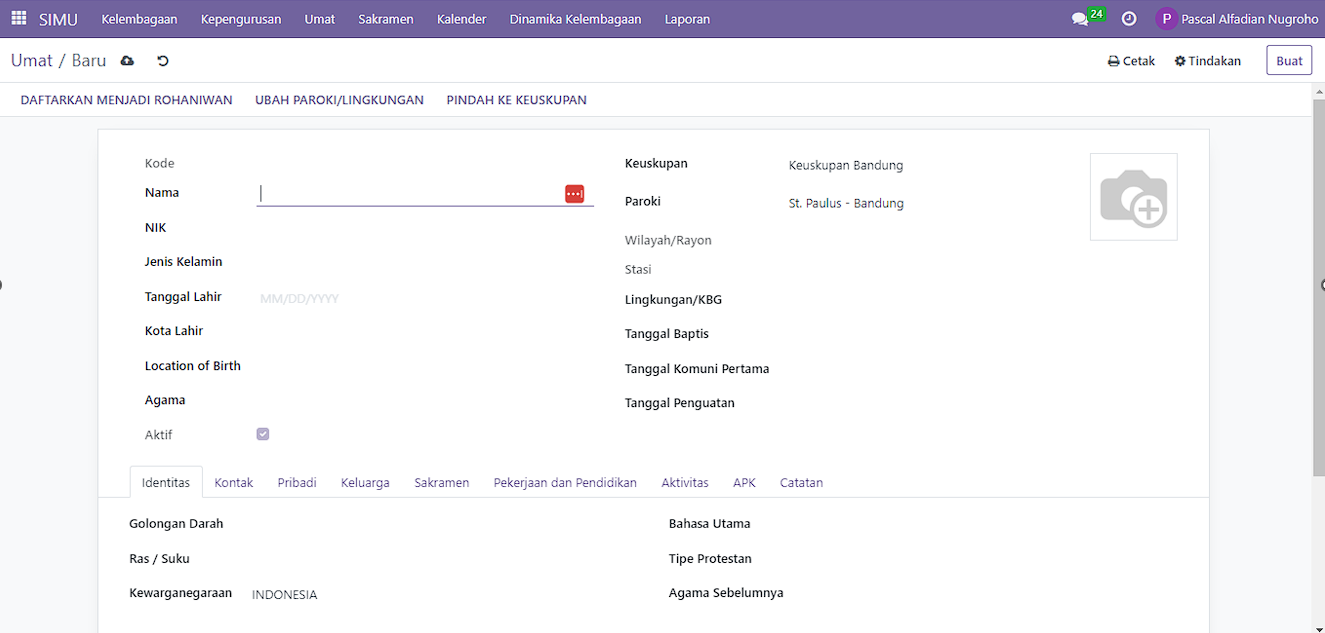
\includegraphics[scale=0.6]{Gambar/simuInput.png}
	\caption{Contoh Menu Input Data Baru SIMU} 
	\label{fig:simuInput}
\end{figure}

Apabila keluarga juga belum tercatat di SIMU, maka admin harus memasukkan juga data keluarga melalui menu Umat > Keluarga Katolik dan klik “Buat”. Admin perlu mengisikan seluruh data yang ada ke dalam formulir, dan klik Simpan.

\begin{figure}[H]
	\centering
	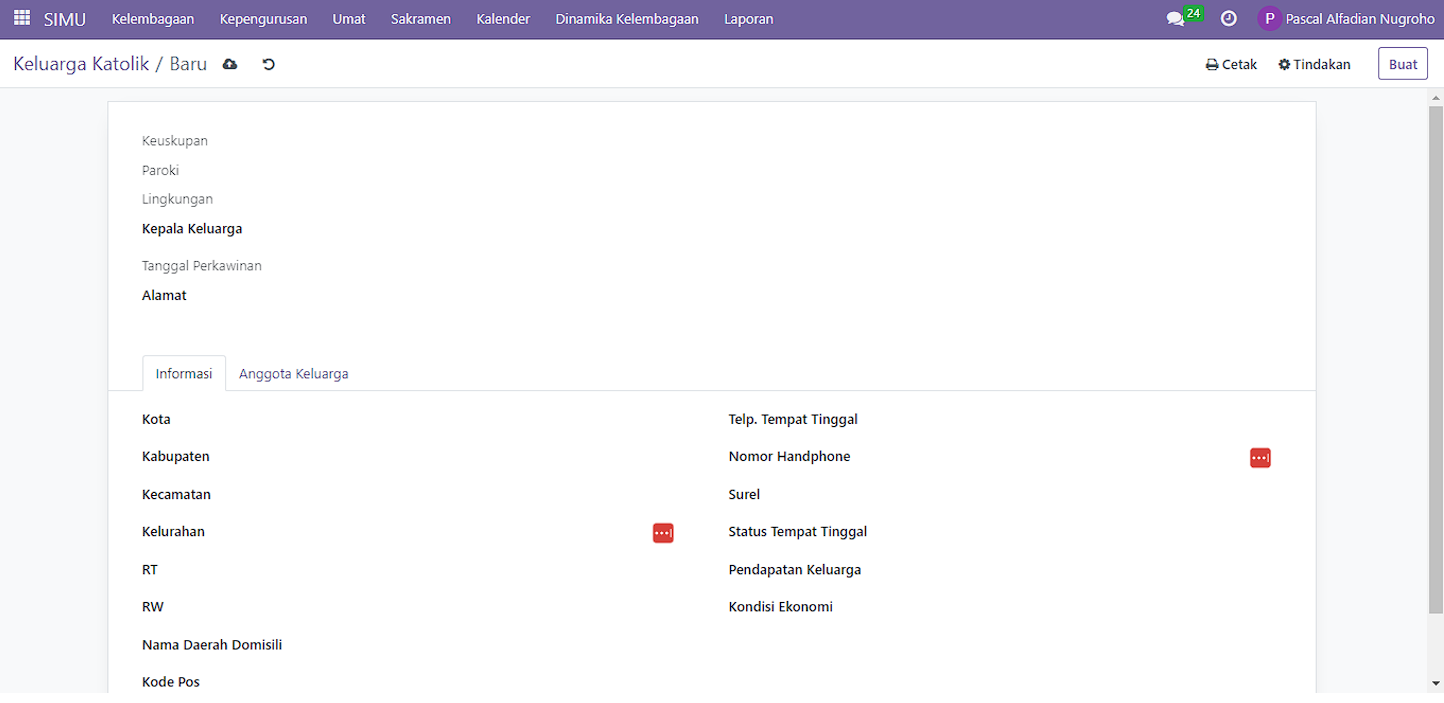
\includegraphics[scale=0.55]{Gambar/simuKeluarga.png}
	\caption{Contoh Input Data Baru Keluarga Katolik} 
	\label{fig:simuKeluarga}
\end{figure}

\begin{figure}[H]
	\centering
	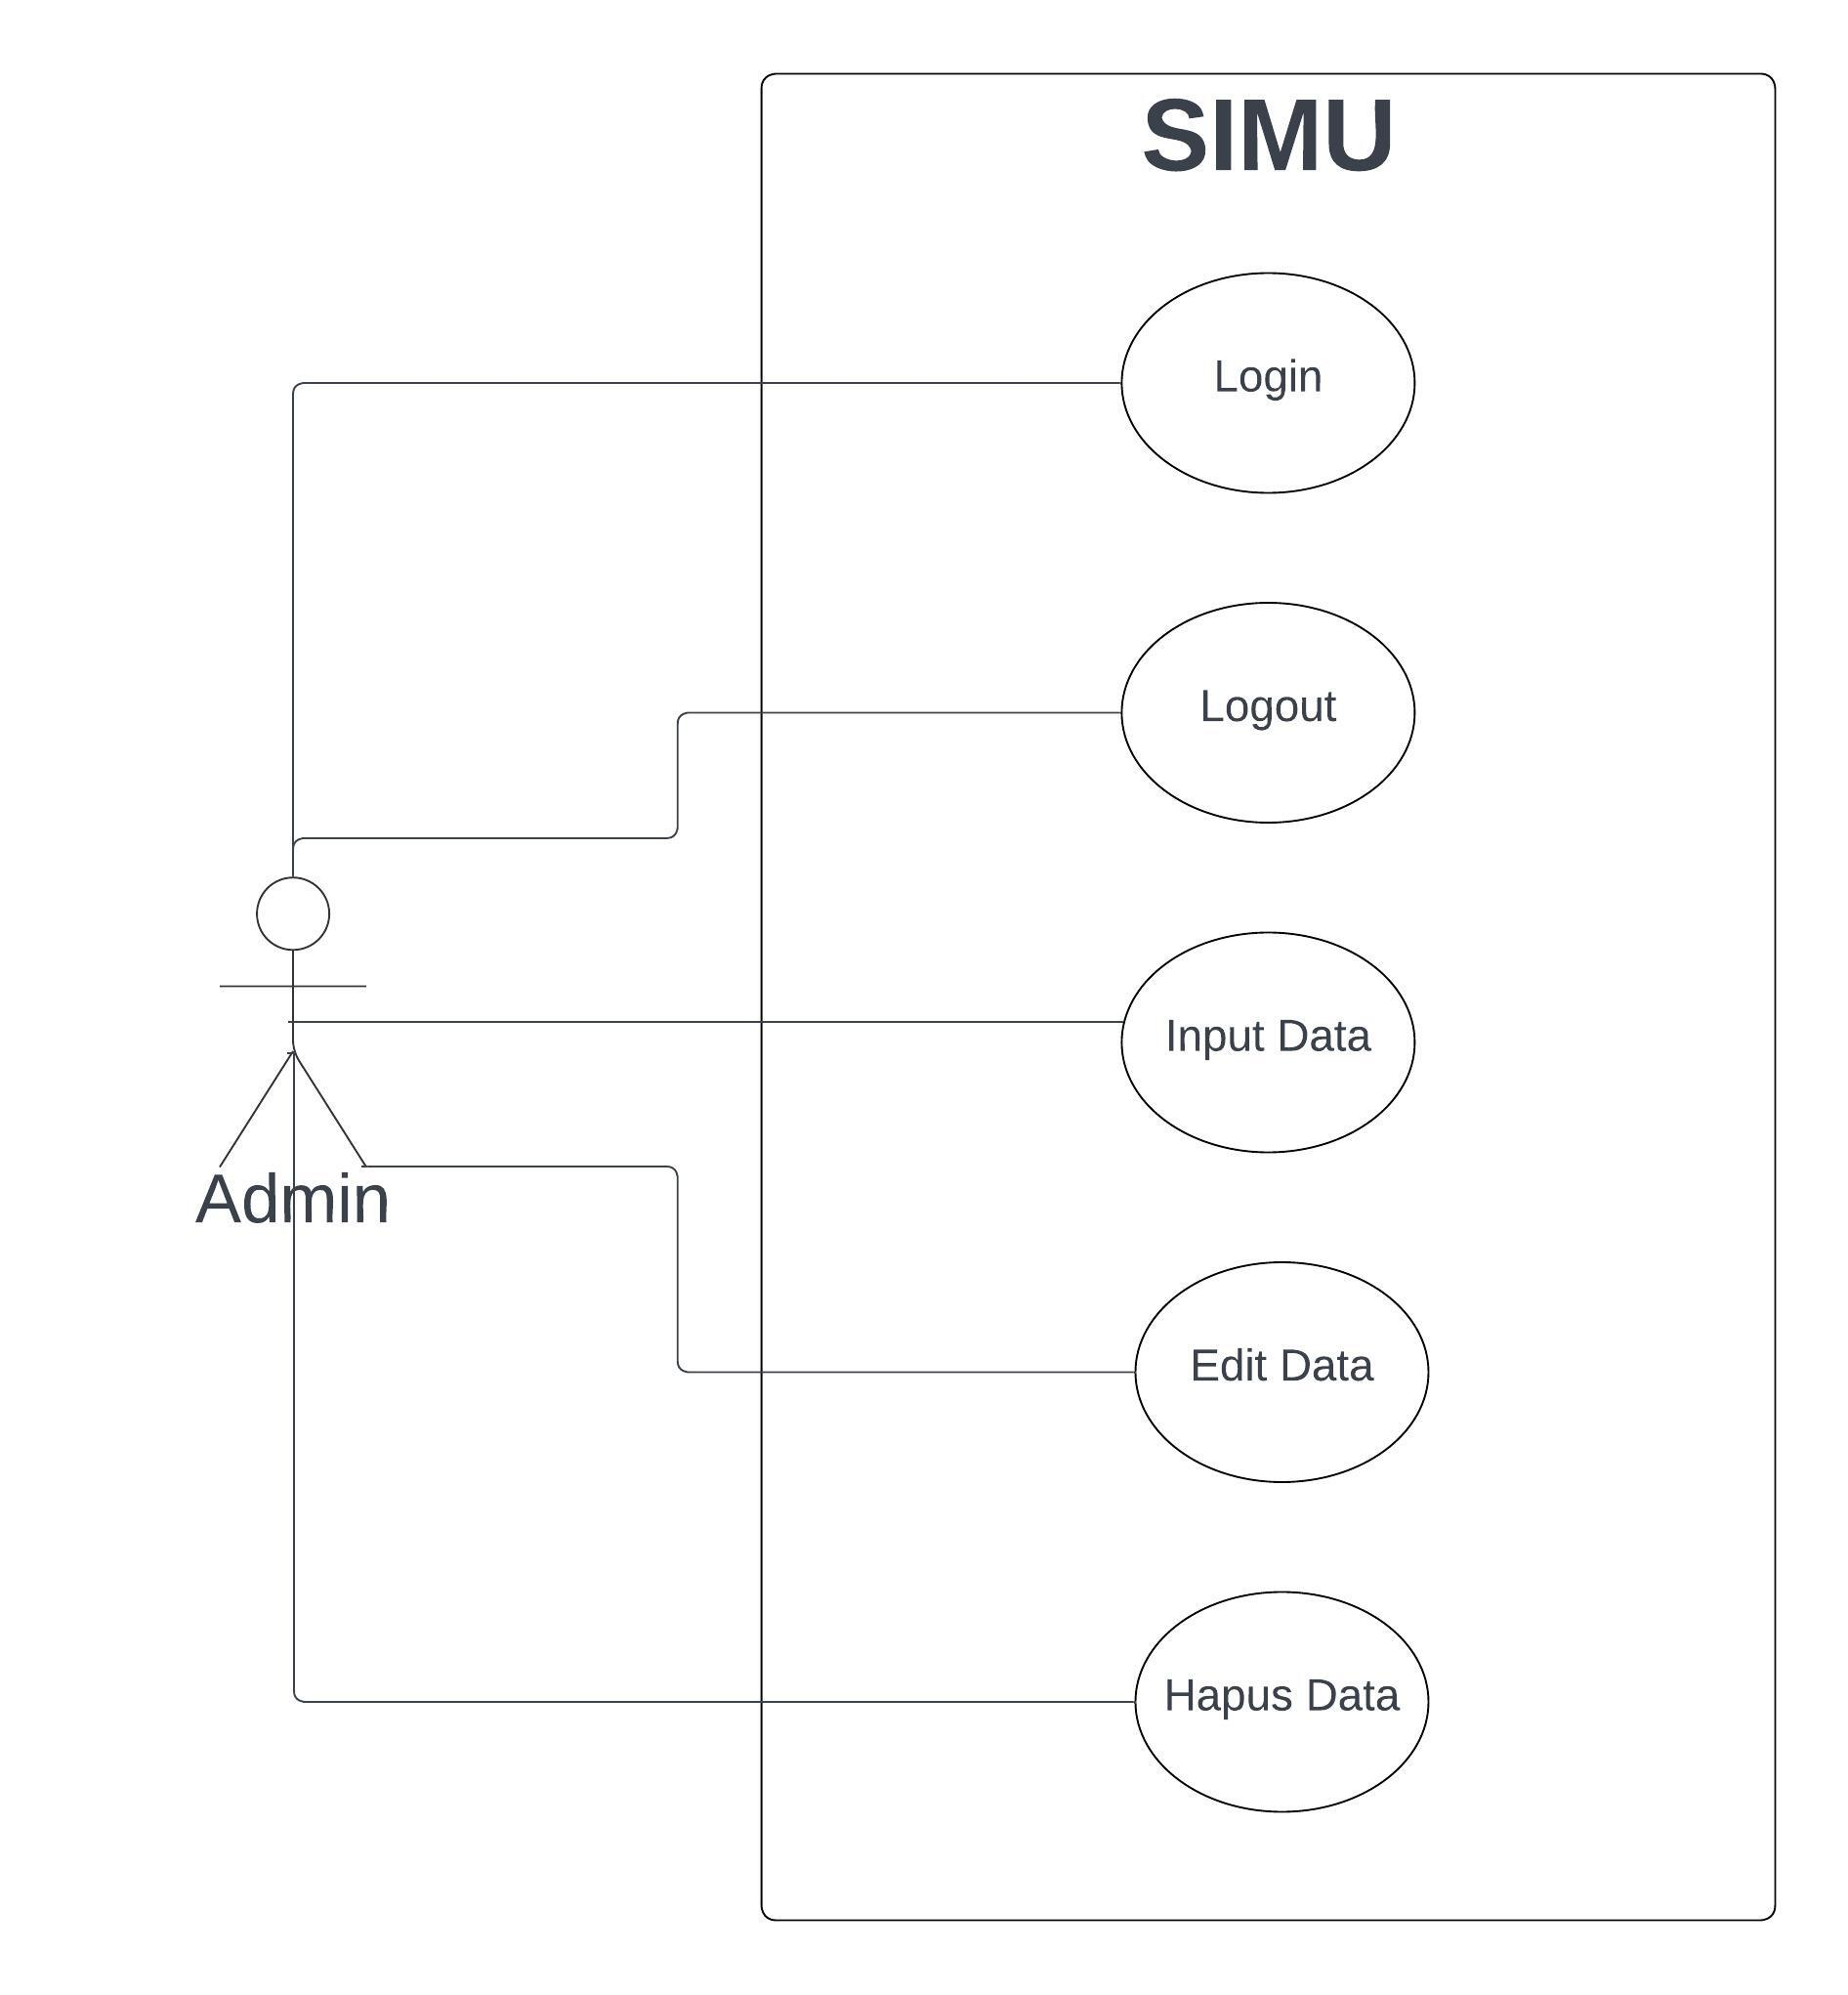
\includegraphics[scale=0.7]{Gambar/usecaseAdmin.jpeg}
	\caption{Diagram Use Case SIMU} 
	\label{fig:usecaseAdmin}
\end{figure}

Setelah penggambaran use case diagram perlu dijelaskan skenario dari use case diagram tersebut. Skenario use case merupakan alur jalannya proses use case dari sisi admin maupun sistemnya. Berikut ini merupakan skenario use case yang disajikan dalam bentuk tabel.

Pada Gambar \ref{fig:simuInput} adalah tampilan awal ketika masuk ke halaman SIMU untuk bagian menu Umat Baru. Fitur-fitur yang tersedia pada SIMU sebagai berikut:

\begin{enumerate}
	\item \textit{Login}: Untuk dapat menggunakan situs SIMU, admin harus \textit{login} menggunakan \textit{email} dan \textit{password} milik admin tersebut.
	\begin{itemize}
		\item Nama Use Case: \textit{Login}
		\item Aktor: Admin
		\item Deskripsi: \textit{Login} ke SIMU.
		\item Kondisi awal: Belum \textit{login}.
		\item Kondisi akhir: Halaman utama SIMU.
		\item Skenario utama:
		\begin{table}[h!]
			\centering
			\label{}
			\begin{tabular}{ | m{0.5cm} | m{7cm}| m{6cm} | } 
				\hline
				No & Aksi Aktor & Reaksi Sistem \\ 
				\hline
				1 & Admin mengakses SIMU & Sistem menampilkan halaman \textit{login}.
				\\ 
				\hline
				2 & Admin mengisi \textit{email} dan \textit{password} lalu menekan tombol ``Login'' & Sistem menampilkan halaman utama SIMU.
				\\ 
				\hline
				3 & Admin mengakses halaman Umat > Umat lalu menekan tombol klik & Sistem menampilkan halaman Umat Baru.
				\\ 
				\hline
			\end{tabular}
		\end{table}

\newpage

\subsection{Fitur Tambahan Pemanfaatan QR Code dalam Input Data Odoo, Studi Kasus: SIMU}

\begin{figure}[H]
	\centering
	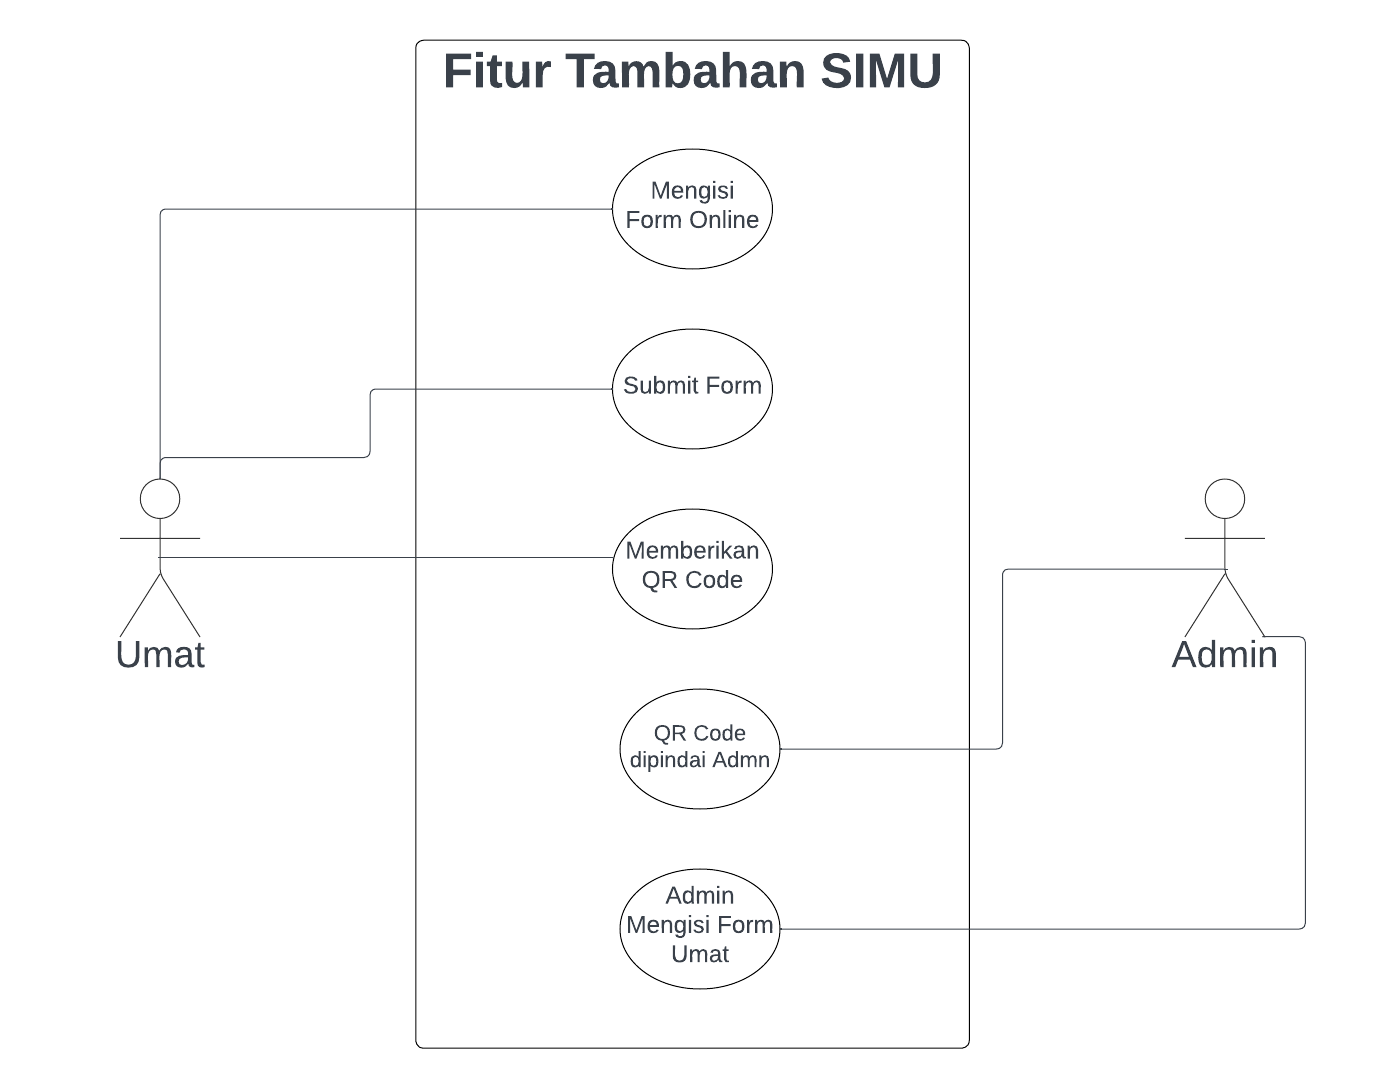
\includegraphics[scale=0.7]{Gambar/fiturTambahan.png}
	\caption{Diagram Use Case Fitur Tambahan SIMU} 
	\label{fig:fiturTambahan}
\end{figure}

Skenario use case ini merupakan tambahan lanjutan fitur dari use case pada subbab \ref{sec:inputDataBaru} yang tidak memiliki fitur tambahan input data secara online melalui form website.

\newpage

\section{Analisis Sistem Usulan}
\label{sec:analisisSistemusulan}

\subsection{Anilisis Hasil Survei Input Data Melalui Formulir Manual dan Formulir Online}

Survei input data umat baru dilakukan untuk mengetahui berapa lama waktu yang dibutuhkan untuk melakukan input data umat baru secara manual melalui kertas yang sudah dicetak ataupun secara online melalui formulir website. Survei ini baru saja diberikan kepada teman mahasiswa penulis skripsi dan dosen Teknik Informatika Universitas Katolik Parahyangan, dosen tersebut merupakan Dosen Pembimbing saya yaitu Pascal Alfadian, Nugroho, M.Comp. Hasil survei menunjukan bahwa waktu yang dibutuhkan untuk melakukan pengisian data lebih cepat menggunakan formulir online, karena pada pengisan data tersebut dapat dilakukan dimana saja, tanpa harus mengambil terlebih dahulu kertas formulir yang sudah dicetak. Pada pengisian formulir online juga terdapat fitur \textit{save} dan \textit{load} sehingga apabila \textit{browser} formulir tertutup ataupun umat mau mengisinya dilain waktu, data yang sudah diisi akan tersimpan didalam \textit{cookies}. Formulir online ini juga bermanfaat karena dapat mengurangi tingkat kesalahan dalam penulisan data umat.

\begin{figure}[H]
	\centering
	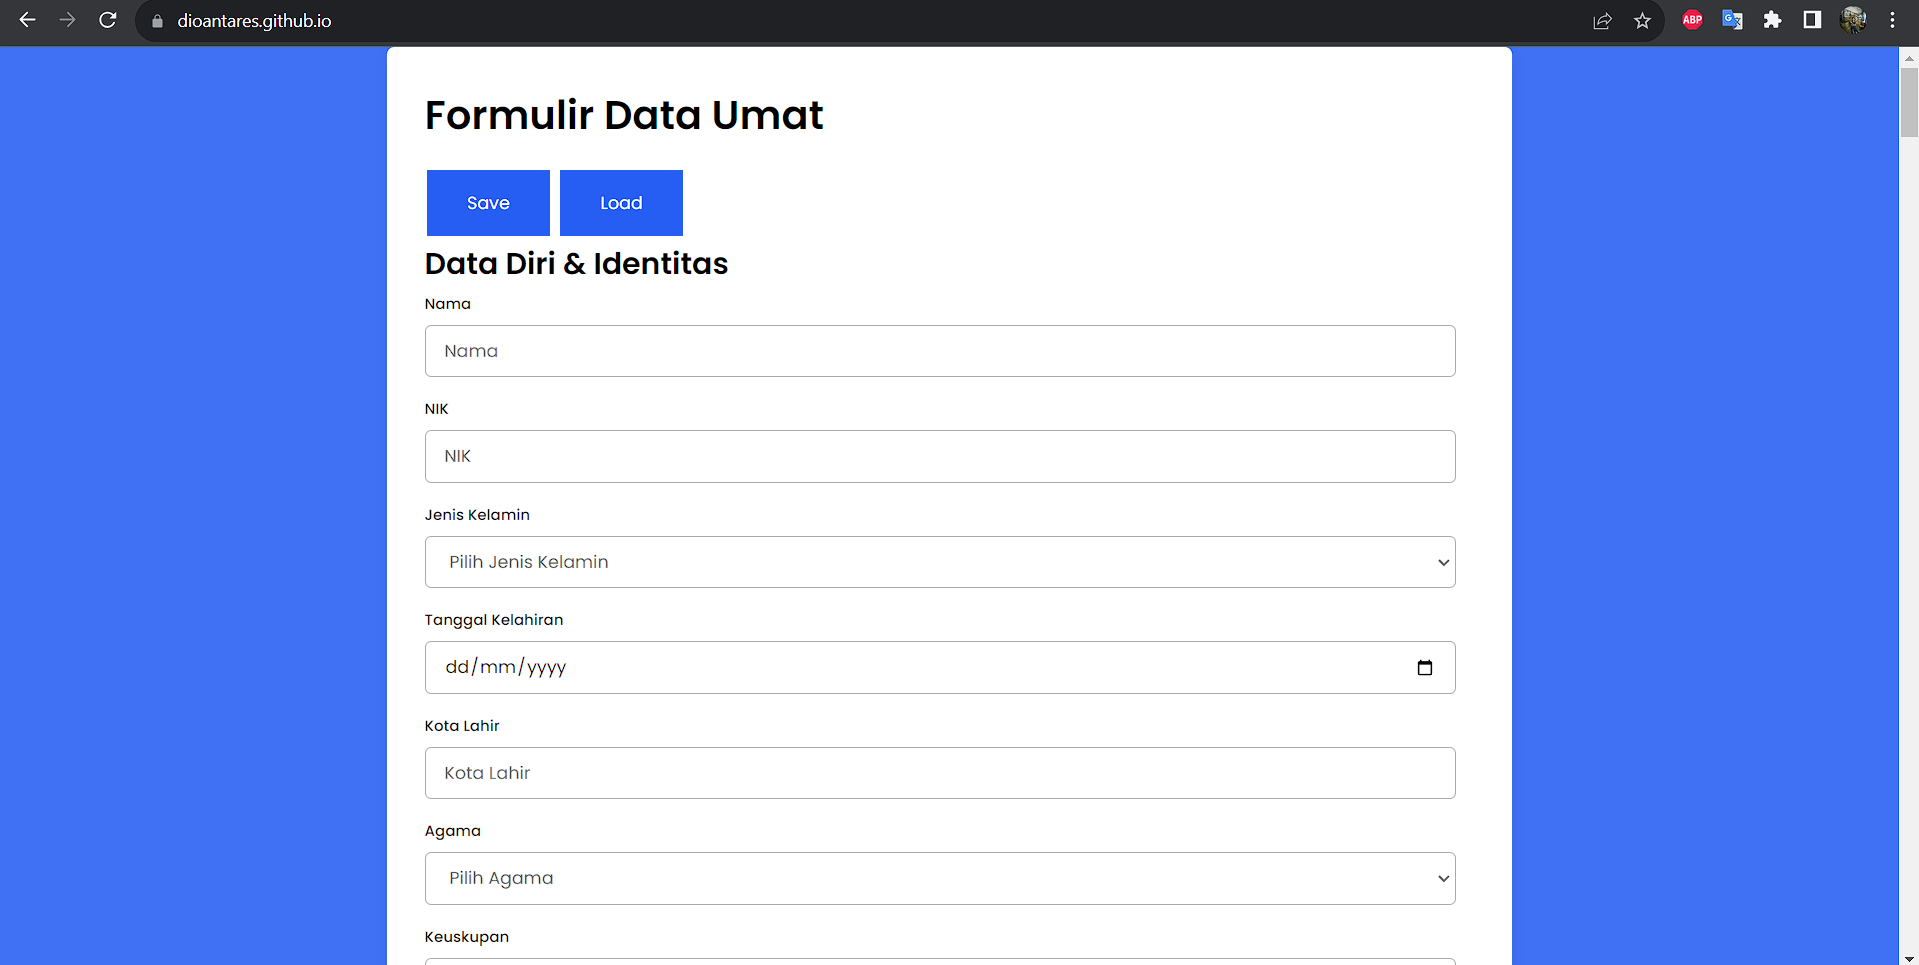
\includegraphics[scale=0.7]{Gambar/formUmat.png}
	\caption{Tombol Save dan Load untuk formulir Umat} 
	\label{fig:loadSave}
\end{figure}

Pada gambar \ref{fig:loadSave} merupakan contoh formulir online untuk pengisian data umat baru, tersedianya fitur \textit{save} dan \textit{load} agar umat tidak perlu mengisi kembali dari awal apabila browser tertutup ataupun umat ingin melanjutkan mengisi kembali formulir dilain waktu, salah satu alasan lainnya adalah karena formulir ini cukup banyak yang perlu diisi, apabila tidak terdapat fitur ini, maka umat akan mengulangi pengisian data dari awal, sehingga akan memakan waktu yang lebih banyak.

\begin{figure}[H]
	\centering
	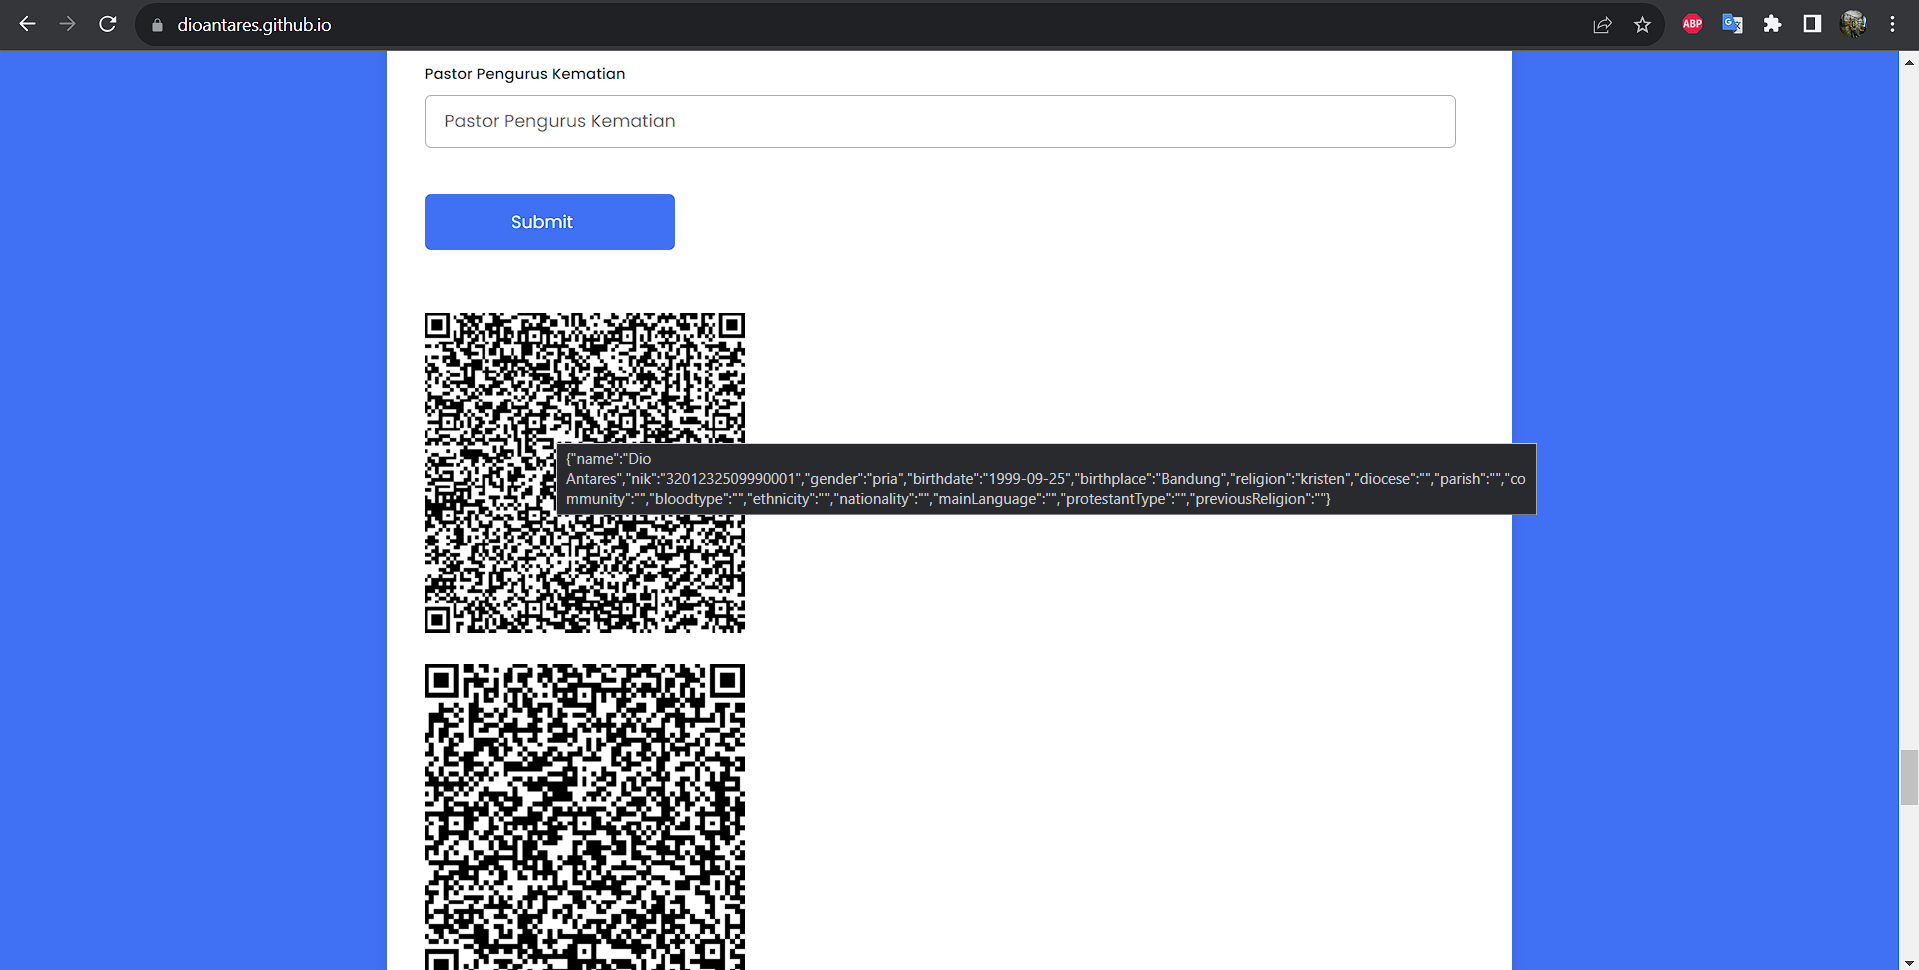
\includegraphics[scale=0.7]{Gambar/qrCodeSubmit.png}
	\caption{QR Code dari data yang telah diisi} 
	\label{fig:qrCodeSubmit}
\end{figure}

Pada gambar \ref{fig:qrCodeSubmit} merupakan hasil QR Code yang dihasilkan dari data yang telah diisi pada formulir. Setelah umat mengisi data, umat harus klik \textit{submit} sehingga website akan mengeluarkan beberapa QR Code yang sudah dibagi menjadi beberapa bagian. Pada gambar tersebut hanya mengeluarkan data yang berisi nama dengan \textit{value} "Dio". 